%!TEX root = ../../thesis.tex

\section{Further Advances}
\label{sec:advances}

In this section, we summarize recent advances in neural reading comprehension. We divide them into the following four categories: {word representations}, {attention mechanisms}, {alternatives to LSTMs}, and {others} (such as training objectives, data augmentation). We give a summary and discuss their importance in the end.


\subsection{Word Representations}
The first category is better word representations for question and passage words, so the neural models are built off of better grounds. Learning better distributed word representations from text or finding the best set of word embeddings for specific tasks still remains an active research topic --- for example, \newcite{mikolov2017advances} find that replacing \sys{GloVe} pre-trained vectors with the new \sys{fastText} vectors~\cite{bojanowski2017enriching} in our model brings about 1 point of improvement on \sys{SQuAD}. More than that, there are two key ideas which have been proved (highly) useful:

\subsubsection*{Character embeddings}
The first idea is to use character-level embeddings to represent words, which are especially helpful for rare or out-of-vocabulary words. Most of the existing works employ a \sys{convolutional neural network} (CNN), which can usefully exploit the surface patterns of $n$-gram characters. More concretely, let  $\mathcal{C}$ be the vocabulary of characters and each word type $x$ can be represented as a sequence of characters $(c_1, \ldots, c_{|x|}), \forall c_i \in \mathcal{C}$. We first map each character in $\mathcal{C}$ into a $d_c$-dimensional vector, so word $x$ can be represented as $\mf{c}_1, \ldots, \mf{c}_{|x|}$.

Next we apply a convolution layer with a filter $\mf{w} \in \R^{d_c \times w}$ of width $w$, and we denote $\mf{c}_{i:i+j}$ as the concatenation of $\mf{c}_i, \mf{c}_{i + 1}, \ldots, \mf{c}_{i + j}$. Therefore, for $i = 1, \ldots, |x| - w + 1$, we can apply this filter $\mf{w}$ and after which we add a bias $b$ and apply a nonlinearity $\tanh$ as follows:
\begin{equation}
    f_i = \tanh\left(\mf{w}^{\intercal} \mf{c}_{i:i+w-1} + b \right).
\end{equation}
Finally we can apply a \ti{max-pooling} operation on $f_1, \ldots, f_{|x| - w + 1}$ and obtain one scalar feature:
\begin{equation}
    f = \max_{i}{\{f_i\}}
\end{equation}
This feature essentially picks out a character $n$-gram, where the size of the $n$-gram corresponds to the filter width $w$. We can repeat the above process by repeating $d^*$ different filters $\mf{w}_1, \ldots, \mf{w}_{d^*}$. As a result, we can obtain a character-based word representation for each word type $\mf{E}_c(x) \in \R^{d^*}$. All the character embeddings, filter weights $\{\mf{w}\}$ and biases $\{b\}$ are learned during training. More details can be found in \newcite{kim2014convolutional}.  In practice, the dimension of character embeddings $d_c$ usually takes a small value (e.g., 20), width $w$ usually takes $3 - 5$, while $100$ is a typical value for $d^*$.

\subsubsection*{Contextualized word embeddings}
Another important idea is \ti{contextualized word embeddings}. Different from traditional word embeddings in which each word type is mapped to one single vector, contextualized word embeddings assign each word a vector as a function of the entire input sentence. These word embeddings can model better complex characteristics of word use (e.g., syntax and semantics) and how these uses vary across linguistic contexts (i.e., polysemy).

A concrete implementation is \sys{ELMo} detailed in \newcite{peters2018deep}: their contextualized word embeddings are learned functions of the internal states of a deep bidirectional language model, which is pretrained on a large text corpus. Basically, given a sequence of words $(x_1, x_2, \ldots, x_n)$, they run an $L$-layer forward LSTM and models the sequence probability as:
\begin{equation}
    P(x_1, x_2, \ldots, x_n) =  \prod_{k = 1}^{n}P(x_k \mid x_1, \ldots, x_{k - 1})
\end{equation}
Only the top layer of the LSTM $\overrightarrow{\mf{h}}^{(L)}_k$ is used to predict the next token $x_{k + 1}$. Similarly, another $L$-layer LSTM is run backward and $\overleftarrow{\mf{h}}^{(L)}_k$ is used to predict the token $x_{k - 1}$. The overall training objective is to maximize the log-likelihood from both directions:
\begin{equation}
  \small
    \sum_{k=1}^{n}\left({\log P (x_k \mid x_1, \ldots, x_{k-1}; {\Theta}_x, \overrightarrow{{\Theta}}_{\text{LSTM}}, {\Theta}_s ) + \log P (x_k \mid x_{k+1}, \ldots, x_{n}; {\Theta}_x, \overleftarrow{{\Theta}}_{\text{LSTM}}, {\Theta}_s )}\right),
\end{equation}
where $\Theta_x$ and $\Theta_s$ are word embeddings and softmax parameters and shared for both LSTMs. The final contextualized word embeddings are computed as a linear combination of all the biLSTM layers and the input word embeddings, multiplied by a linear scalar:
\begin{equation}
    \sys{ELMo}(x_k) = \gamma \left(s_0 \mf{x}_k + \sum_{j=1}^{L}{\overrightarrow{s}_{j} \overrightarrow{\mf{h}}^{(j)}_k} + \sum_{j=1}^{L}{\overleftarrow{s}_{j} \overleftarrow{\mf{h}}^{(j)}_k} \right)
\end{equation}
All the weights $\gamma, s_0, \overrightarrow{s}_{j}, \overleftarrow{s}_{j}$ are task-specific and learned during the training process.

These contextualized word embeddings are usually used in conjunction with traditional word type embeddings and character embeddings. It turns out that this sort of contextualized word embeddings pre-trained on very large text corpora (e.g., 1B Word Benchmark~\cite{chelba2014one}) has been highly effective. \newcite{peters2018deep} demonstrated that adding ELMo embeddings ($L = 2$ biLSTM layers with $4096$ units and $512$ dimension projections) to an existing competitive model can bring the F1 score on \sys{SQuAD} from $81.1$ to $85.8$ directly, a $4.7$ point of absolute improvement.

Earlier than \sys{Elmo}, \newcite{mccann2017learned} proposed \sys{CoVe}, which learned contextualized word embeddings in a neural machine translation framework, and the resulting encoder can be used in a similar way as an addition to the word embeddings. They also demonstrated a $4.3$ point of absolute improvement on \sys{SQuAD}.

Very recently, \newcite{radford2018improving} and \newcite{devlin2018bert} find that these contextualized word embeddings can not only be used as features of word representations in a task-specific neural architecture (a reading comprehension model in our context), but we can fine-tune the deep language models directly with minimal modifications to perform downstream tasks. This is indeed a very striking result at the time of writing this thesis and we will discuss it more in Section~\ref{sec:rep-vs-arch} and there still remain many open questions to answer in the future. Additionally, \newcite{devlin2018bert} proposed a clever way to train bidirectional language models: instead of always stacking LSTMs in one direction and predicting the next word,\footnote{To make it clear, although ELMo adopts a biLSTM, it is essentially the use of two unidirectional LSTMs for predicting the next word in both directions.} they mask out some words at random at the input layer, stack bidirectional layers and predict these masked words at the top layer. They find this training strategy extremely useful empirically.

\subsection{Attention Mechanisms}
\label{sec:attention-mechanisms}

There have been a multitude of attention variants proposed for neural reading comprehension models, and they aim to capture semantic similarity between the question and the passage, at different levels, multiple granularity, or in a hierarchical way. A typical complex example in this direction can be found at \cite{huang2018fusionnet}. To our best knowledge, there isn't a conclusion yet if there is one single variant that stands out. Our \sys{Stanford Attentive Reader} (Section~\ref{sec:sar}) takes the most simple possible form of attention (Figure~\ref{fig:att-overview} illustrates an overview of different layers of attention). Besides that, we think there are two ideas which can generally further improve the performance of these systems:

\begin{figure}[t]
\centering
\vspace{1em}
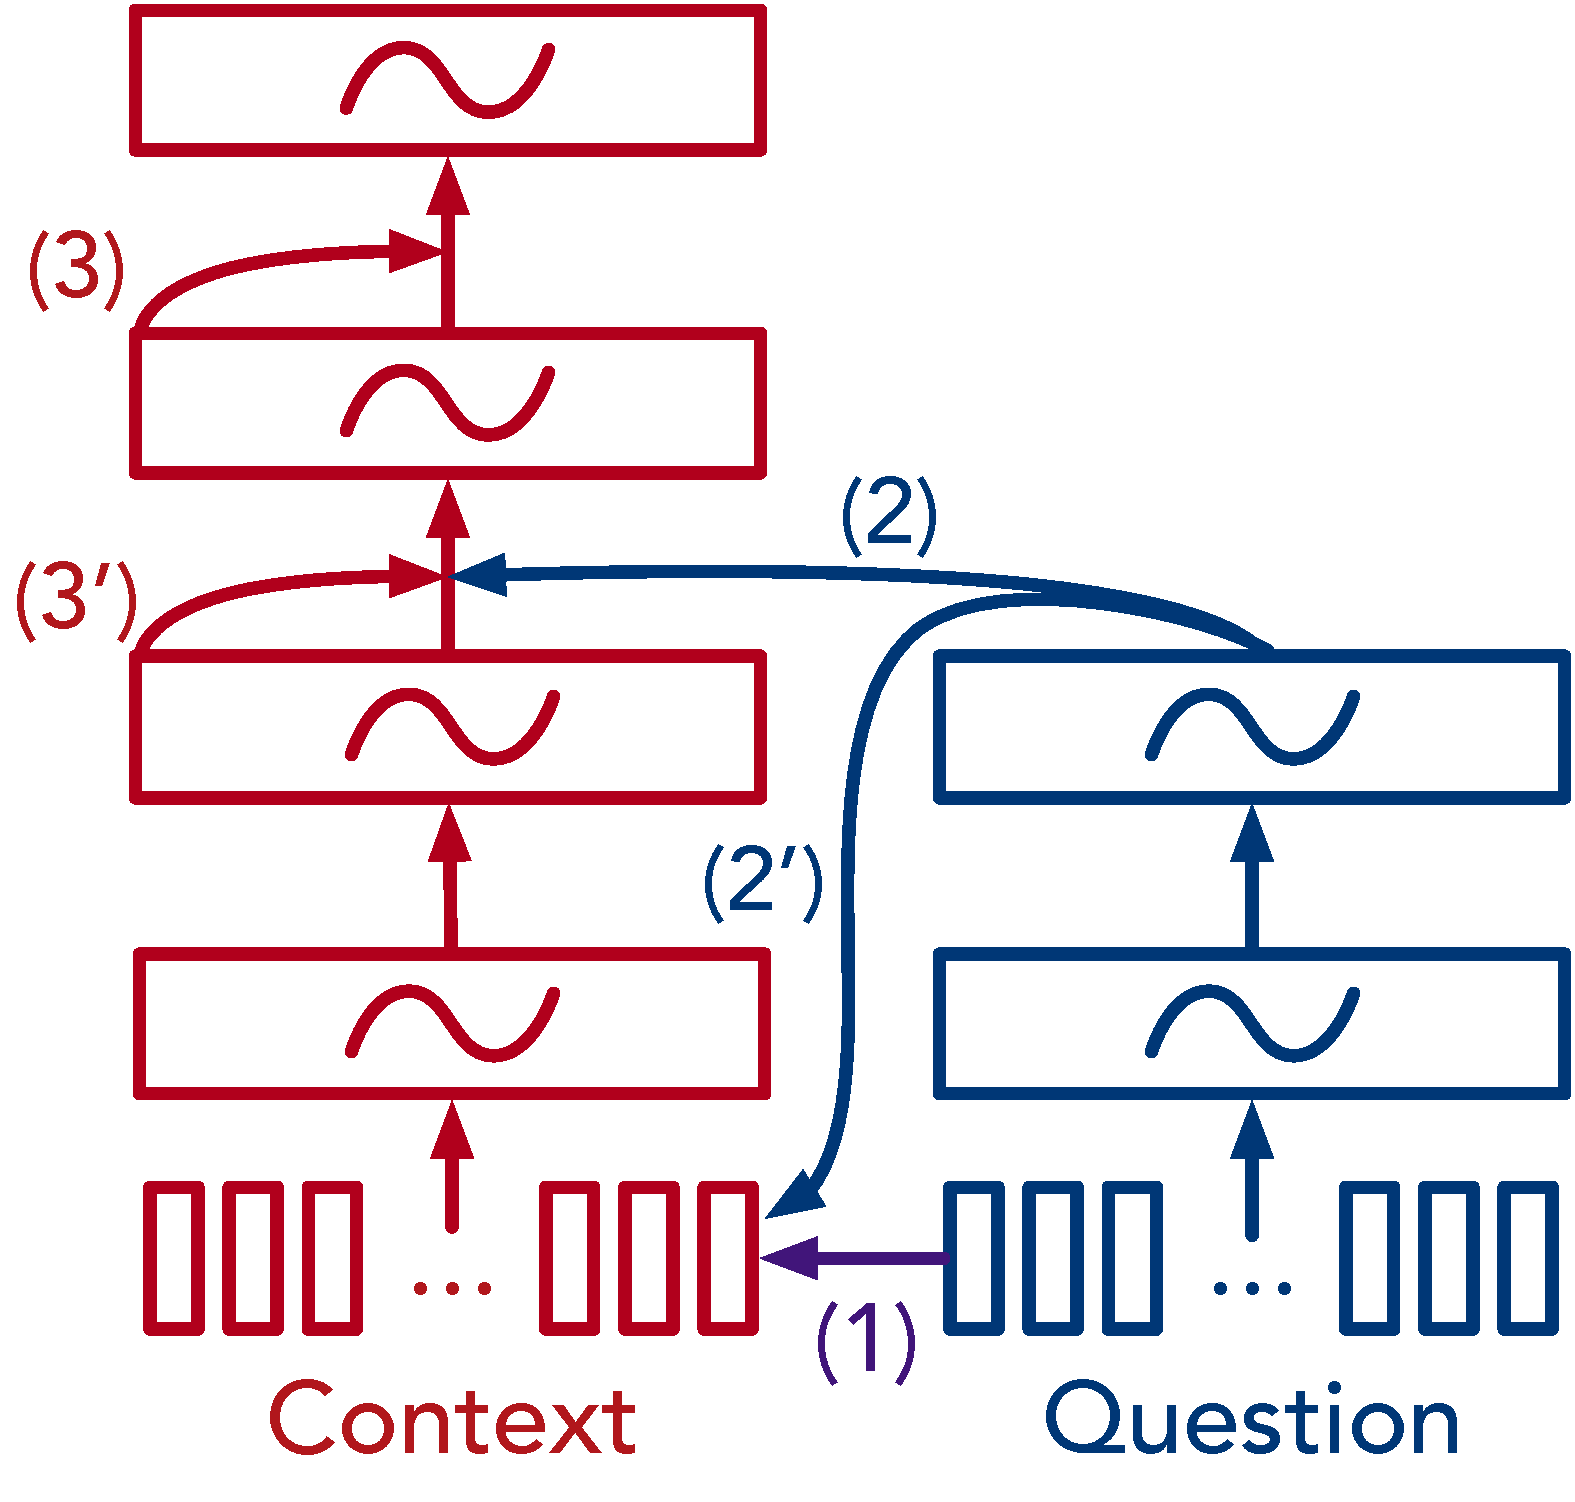
\includegraphics[scale=0.25]{img/gen_fusion.pdf}
\vspace{1em}

\begin{tabular}{l|ccccc}
\hline
\bf Architectures & \bf (1) & \bf (2) & \bf (2') & \bf (3) & \bf (3') \\ \hline
Match-LSTM \citep{wang2017machine} & & \checkmark & & & \\
DCN \citep{xiong2017dynamic} & & \checkmark & & & \checkmark \\
BiDAF \citep{seo2017bidirectional} & & \checkmark & & & \checkmark \\
RaSoR \citep{lee2016learning} & \checkmark & & \checkmark & & \\
R-net \citep{wang2017gated} & & \checkmark & & \checkmark & \\
\hline
Our model & \checkmark & & & &  \\
\hline
\end{tabular}
\longcaption{A summary of different layers of attention.}{\label{fig:att-overview} A summary of different layers of attention. Image courtesy: \cite{huang2018fusionnet} with minimal modifications.}
\end{figure}

\subsubsection*{Bidirectional attention}

\newcite{seo2017bidirectional} first introduced the idea of \ti{bidirectional attention}. In addition to what we already have, the key difference is that they have the \ti{question-to-passage} attention, which signifies which passage words have the closest similarity to each of the question words. In practice, this can be implemented as: for each word in the question, we can compute an attention map over all the passage words, similar as we did in Equation~\ref{eq:aligned_question} and \ref{eq:aligned_question_attention}, but in opposite directions:

\begin{equation}
    f_{q\_align}(q_i) = \sum_j{b_{i, j} \mf{E}(p_j)}.
\end{equation}
After this, we can simply feed $f_{q\_align}(q_i)$ into the input layer of the question encoding (Section~\ref{sec:question-encoding}).

The attention mechanism in \newcite{seo2017bidirectional} is a bit more complex, but we think it is similar. We also argue that the attention function in this direction is less useful, as also demonstrated in \newcite{seo2017bidirectional}. This is because the questions are generally short (10-20 words on average) and using one single LSTM for question encoding (without extra attention) is usually sufficient.

\subsubsection*{Self-attention over passage}
The second idea is \ti{self-attention} over the passage words, first introduced in \newcite{wang2017gated}.\footnote{They named it as ``self-matching attention mechanism'' in the paper.} The intuition is that the passage words can be aligned to the other passage words, with the hope that it can address coreference problems and aggregate information (of the same entity) from multiple places in the passage.

In detail, \newcite{wang2017gated} first compute the hidden vectors for the passage: $\mf{p}_1, \mf{p}_2, \ldots, \mf{p}_{l_p}$ (Equation~\ref{eq:passage-lstm}), and then for each $\mf{p}_i$, they apply an attention function over $\mf{p}_1, \mf{p}_2, \ldots, \mf{p}_{l_p}$ via one hidden layer of MLP (Equation~\ref{eq:mlp-att}):
\begin{eqnarray}
    a_{i, j} & =&  \frac{\exp\left(g_{\text{MLP}}(\mf{p}_i, \mf{p}_j)\right)}{\sum_{j'}\exp\left(g_{\text{MLP}}(\mf{p}_i, \mf{p}_{j'})\right)} \\
    \mf{c}_i & = & \sum_{j}{a_{i, j}\mf{p}_j}
\end{eqnarray}
Later, $\mf{c}_i$ and $\mf{p}_i$ are concatenated and fed into another BiLSTM: $\mf{h}^{(p)}_i = \text{BiLSTM}(\mf{h}^{(p)}_{i-1}, [\mf{p}_i, \mf{c}_i])$, and can be used as the final passage representations.

\subsection{Alternatives to LSTMs}
\label{sec:alt-lstms}
All the models we discussed so far are based on recurrent neural networks (RNNs), in particular, LSTMs. It is well known that increasing the depth of neural networks can improve the capacity of models and bring gains in performance~\cite{he2016deep}. We also discussed earlier that deep BiLSTMs of $3$ or $4$ layers usually perform better than a single layer of BiLSTM (Section~\ref{sec:imp-details}). However, we are facing two challenges as we further increase the depth of the LSTM models: 1) It gets more difficult to optimize due to the vanishing gradient problem; 2) Scalability becomes an issue as the training/inference time increases linearly as the number of layer grows. It is known that LSTMs are difficult to parallelize and thus scale poorly due to their sequential nature.

On the one hand, there are works which attempt to add highway connections~\cite{srivastava2015training} or residual connections~\cite{he2016deep} between layers, so it eases the optimization and enables training more layers of LSTMs. On the other hand, people set out to find replacements for LSTMs, getting rid of recurrent structures while still performing similarly or even better.

The most notable work in this line is the \sys{Transformer} model proposed by Google researchers~\cite{vaswani2017attention}. \sys{Transformer} only builds on top of word embeddings and simple positional encodings with stacked self-attention layers and position-wise fully connected layers. With residual connections, this model is able to be trained fast with many layers. It first demonstrated superior performance on a machine translation task with $L = 6$ layers (each layer consists of a self-attention and a fully connected feedforward network), and then later was adapted by~\cite{yu2018qanet} for reading comprehension.

The model called \sys{QANet} \cite{yu2018qanet} stacks multiple convolutional layers followed by the self-attention and fully connected layer, as a building block, for both question and passage encoding as well as a few more layers stacked before the final prediction. The model demonstrated state-of-the-art performance at the time (Table~\ref{tab:squad-results}) while showing significant speed-ups.

Another research work by \newcite{lei2018simple} proposed a lightweight recurrent unit called \sys{Simple Recurrent Unit} (SRU) by simplifying the LSTM formulation while enabling CUDA-level optimizations for high parallelization. Their results suggest that simplified recurrence retains strong modeling capacity through layer stacking. They also demonstrate that replacing the LSTMs in our model with their \sys{SRU} unit can improve the F1 score by 2 points while being faster for training and inference.

\subsection{Others}

\paragraph{Training objectives.} It is also possible to make further progress by improving the training objectives. It is usually straightforward to employ a cross-entropy or max-margin loss for the cloze style or multiple choice problems. However, for span prediction problems, \newcite{xiong2018dcn+} suggest that there is a discrepancy between the cross-entropy loss of predicting two endpoints of the answer and the final evaluation metrics, which concerns the word overlap between gold answer and ground truth. For the following example:

\begin{displayquote}
\tf{passage}: Some believe that the Golden State Warriors team of 2017 is one of the greatest teams in NBA history \ldots \\
\tf{question}: Which team is considered to be one of the greatest teams in NBA history? \\
\tf{ground truth answer}: the Golden State Warriors team of 2017
\end{displayquote}
Span ``Warriors'' is also a correct answer, however, from the perspective of cross entropy based training it is no better than the span ``history''. \newcite{xiong2018dcn+} propose to use a mixed training objective which combines cross entropy loss over positions and the word overlap measure trained with reinforcement learning. Basically, they use $P^{(\text{start})}(i)$ and $P^{(\text{end})}(i)$ trained with cross-entroy loss to sample the start and end positions of the answer and then use the F1 score as reward function.

For the free-form answer of reading comprehension problems, there has been many recent advances in training better \sys{seq2seq} models especially in the context of neural machine translation, such as sentence-level training~\cite{ranzato2016sequence} and minimum risk training~\cite{shen2016minimum}. However, we don't see many such applications in reading comprehension problems yet.

\paragraph{Data augmentation.} Data augmentation has been a very successful approach for image recognition, while it is less explored in NLP problems. \newcite{yu2018qanet} proposed a simple technique for creating more training data for reading comprehension models. The technique is called \ti{backtranslation} --- basically they leverage two state-of-the-art neural machine translation models: one model from English to French and the other model from French to English, and paraphrase each single sentence in the passage by running through the two models (with some modifications to the answer if needed). They obtained ~2 points gain in F1 by doing this on \sys{SQuAD}. \newcite{devlin2018bert} also find that joint training of \sys{SQuAD} and \sys{TriviaQA}~\cite{joshi2017triviaqa} can help improve the performance on \sys{SQuAD} modestly.

\subsection{Summary}
So far, we have discussed recent advances in different aspects, which, in sum, contribute to the latest progress on current reading comprehension benchmarks (esp. \sys{SQuAD}). Which components are more important than the others? Do we need to add up all of these? Are these recent advances able to generalize to other reading comprehension tasks? How are they correlated with different capacities of language understanding? We think there isn't a clear answer to most of these questions yet and it still requires a lot of investigation.

\begin{table}[!t]
    \centering
    \begin{tabular}{p{6cm} | c l}
    \hline
      \tf{Components} & \tf{F1 improvement} & \tf{References} \\
    \hline
      \sys{Glove}$\Rightarrow$\sys{Fasttext} & 78.9 $\Rightarrow$ 79.8: $+0.9$ & \cite{mikolov2017advances} \\
      Character embeddings & 75.4 $\Rightarrow$ 77.3: $+1.9$ & \cite{seo2017bidirectional} \\
      {\small Contextualized embeddings: \sys{ELMo}} & 81.1 $\Rightarrow$ 85.8: $+4.7$ & \cite{peters2018deep} \\
    \hline
      Question to passage attention & 73.7 $\Rightarrow$ 77.3: $+3.6$ & \cite{seo2017bidirectional} \\
      Self-attention over passage & 76.7 $\Rightarrow$ 79.5: $+2.8$ & \cite{wang2017gated} \\
    \hline
      3-layer LSTMs $\Rightarrow$ 6-layer SRUs & 78.8 $\Rightarrow$ 80.2: $+1.4$ & \cite{lei2018simple} \\
    \hline
      Mixed training objective & 82.1 $\Rightarrow$ 83.1: $+1.0$ & \cite{xiong2018dcn+} \\
      Data augmentation & 82.7 $\Rightarrow$ 83.8: $+1.1$ & \cite{yu2018qanet} \\
    \hline
    \end{tabular}
    \longcaption{A summary of recent advances on \sys{SQuAD}}{\label{tab:impr-squad} A summary of recent advances on \sys{SQuAD}. The numbers are taken from the corresponding papers, on the development set of \sys{SQuAD}.}
\end{table}

We compiled the improvements of different components on \sys{SQuAD} in Table~\ref{tab:impr-squad}. We would like to caution readers that these numbers are really not directly comparable, as they are built on different model architectures and different implementations. We hope that this table at least reflects some ideas regarding the importance of these components on the \sys{SQuAD} dataset. As is seen, all these components contribute to the final performance, more or less. The most important innovation is probably the use of contextualized word embeddings (e.g., \sys{ELMo}), while the formulation of attention functions is also crucial. It will be important to investigate whether these advances can generalize to other reading comprehension tasks in the future.
